\documentclass[11pt,a4paper]{report}
\usepackage[utf8]{inputenc}
\usepackage[spanish]{babel}
\usepackage{geometry}
\geometry{top=2.2cm,bottom=2.2cm,left=2.5cm,right=2.5cm}
\usepackage{fancyhdr}
\usepackage{graphicx}
\graphicspath{{../04 Mapas/}}
\usepackage{booktabs}
\usepackage{tabularx}
\usepackage{xcolor}
\usepackage{float}
\usepackage{titlesec}
\usepackage{amsmath,amssymb}

\definecolor{navyblue}{RGB}{31,78,121}
\definecolor{darkslate}{RGB}{47,85,151}

\titleformat{\chapter}[display]
  {\normalfont\bfseries\color{navyblue}}
  {\filleft\Huge\textbf{\chaptertitlename\ \thechapter}}
  {1ex}
  {\titlerule\vspace{1ex}\LARGE}
  [\vspace{1ex}\titlerule]

\pagestyle{fancy}
\fancyhf{}
\rhead{\small\textcolor{darkslate}{Anexo G: Usos Productivos y Desarrollo Local}}
\lhead{\small\textcolor{darkslate}{MCH Río Blanco 100 kW - Puno}}
\rfoot{\small Página \thepage}
\lfoot{\small UNAP - FIME / Consultoría Energética}

\begin{document}

\begin{titlepage}
\begin{center}
    \vspace*{2cm}
    {\Large\bfseries UNIVERSIDAD NACIONAL DEL ALTIPLANO PUNO}\\[0.5em]
    {\large FACULTAD DE INGENIERÍA MECÁNICA ELÉCTRICA}\\[2.5cm]

    \rule{\linewidth}{2pt}\\[0.4cm]
    {\huge\bfseries\color{navyblue} ANEXO G: ESTUDIO DE APLICACIONES, USOS PRODUCTIVOS DE LA ENERGÍA Y DESARROLLO ECONÓMICO LOCAL}\\[0.4cm]
    {\Large\bfseries PROYECTO MICROCENTRAL HIDROELÉCTRICA RÍO BLANCO 100 kW}\\[0.4cm]
    {\large Distrito de Ollachea, Provincia de Carabaya, Departamento de Puno}\\[0.4cm]
    \rule{\linewidth}{2pt}\\[2.5cm]

    \textbf{Cadenas Productivas Analizadas:}\\
    Agroindustria de Café de Especialidad y Cacao de Altura\\
    Cadena de Frío y Oxigenación para Acuicultura de Truchas\\
    Centro de Transformación Textil de Fibra de Alpaca y Ovino\\
    Bombeo de Agua Potable y Riego Tecnificado en Andenerías\\
    Electromovilidad Rural e Interconexión a Red SEIN (D.L. 1002)\\[2cm]

    \vfill
    {\large Puno -- Perú}\\[0.3em]
    {\normalsize Setiembre 2024 / 2026}
\end{center}
\end{titlepage}

\chapter{Estrategia de Usos Productivos de la Energía Eléctrica}
\section{Justificación del Desarrollo Agroindustrial}
El suministro continuo, estable y económico de energía eléctrica proveniente de la MCH Río Blanco representa un motor de reactivación económica para Ollachea. La potencia instalada neta de 100 kW se ha distribuido estratégicamente para compatibilizar la cobertura residencial con cinco nodos productivos clave.

\begin{figure}[H]
\centering
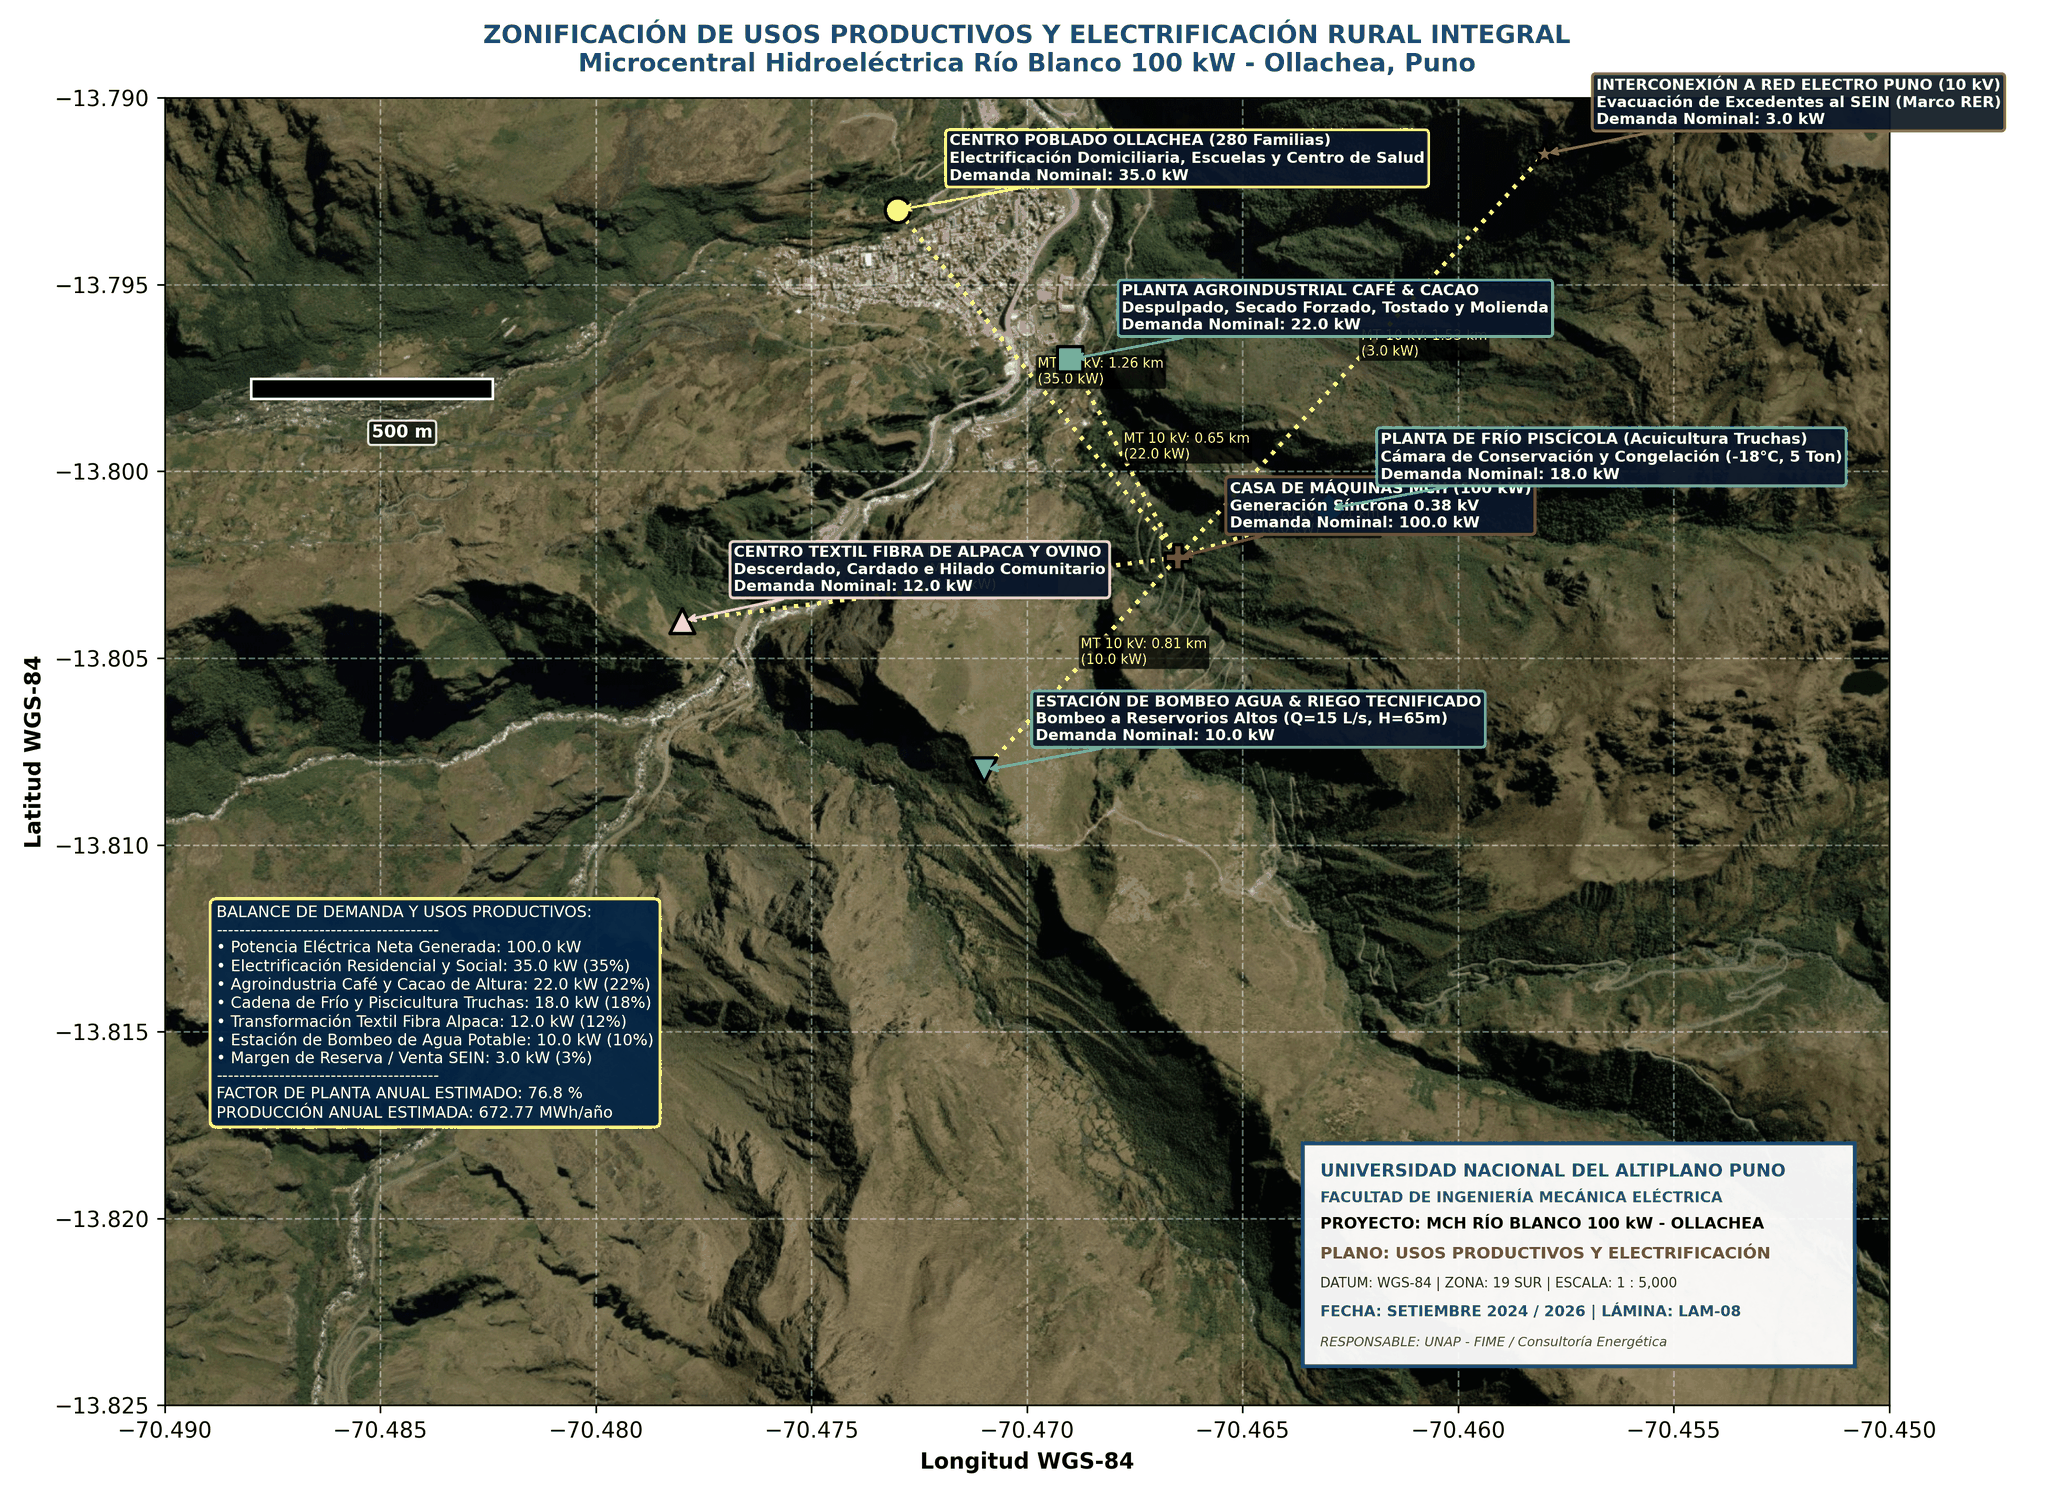
\includegraphics[width=\linewidth]{Mapa_08_Zonificacion_Usos_Productivos_Electrificacion.png}
\caption{Plano de Zonificación de Usos Productivos, Líneas de Distribución 10 kV y Centros de Carga.}
\end{figure}

\section{Balance Integral de Cargas Productivas}
\begin{table}[H]
\centering
\small
\begin{tabularx}{\linewidth}{Xccc}
\toprule
\textbf{Nodo de Consumo Productivo} & \textbf{Potencia [kW]} & \textbf{Consumo [MWh/año]} & \textbf{Horario Principal} \\
\midrule
Electrificación Domiciliaria (280 Familias) & 35.0 kW & 153.30 MWh & 18:00 -- 23:00 hrs \\
Planta de Café y Cacao de Especialidad & 22.0 kW & 115.60 MWh & 08:00 -- 17:00 hrs \\
Cadena de Frío Piscícola (Truchas) & 18.0 kW & 126.14 MWh & 24 Horas continuas \\
Centro de Acopio y Textil de Alpaca & 12.0 kW & 52.56 MWh & 08:00 -- 16:00 hrs \\
Estación de Bombeo de Agua Potable & 10.0 kW & 58.40 MWh & 04:00 -- 07:00 / 13:00 -- 15:00 hrs \\
Margen Operativo y Venta Excedentes SEIN & 3.0 kW & 166.77 MWh & Nocturno / Fin de semana \\
\midrule
\textbf{Total Potencia y Energía Neta Anual} & \textbf{100.0 kW} & \textbf{672.77 MWh/año} & \textbf{Factor de Planta: 76.8\%} \\
\bottomrule
\end{tabularx}
\caption{Matriz de Despacho de Potencia y Energía para Usos Productivos Comunitarios.}
\label{tab:despacho}
\end{table}

\chapter{Ingeniería de Procesos de las Cadenas Productivas}
\section{Agroindustria de Café y Cacao de Especialidad}
Los valles de ceja de selva de Ollachea cuentan con un microclima excepcional para café arábica (\textit{Typica}, \textit{Bourbon} y \textit{Geisha}). El equipamiento electromecánico instalado permitirá el procesamiento con certificación orgánica y denominación de origen:
\begin{itemize}
    \item \textbf{Despulpado Ecológico:} 2 máquinas despulpadoras desmucilaginadoras mecánicas con consumo de agua reducido a menos de 1 litro por kilogramo de café cerezo ($2 \times 3.0\text{ kW}$).
    \item \textbf{Secado Controlado por Convección:} 4 secadores de tambor rotatorio calefaccionados con resistencias eléctricas limpias ($4 \times 2.5\text{ kW}$), reduciendo la humedad del grano de $50\%$ a $11.5\%$ en 24 horas, evitando la fermentación indeseada por lluvias.
    \item \textbf{Módulo de Catación, Tostaduría y Molienda:} Tostador de lecho fluido de 10 kg/batch ($5.0\text{ kW}$) y dos molinos de muelas de titanio ($1.0\text{ kW}$).
\end{itemize}

\section{Cadena de Frío para Acuicultura de Truchas Arcoíris}
El Río Blanco posee aguas prístinas y frías ($9^\circ\text{C}$ a $13^\circ\text{C}$) ideales para el engorde de trucha arcoíris. La infraestructura de conservación garantiza el acceso a mercados de alta gama:
\begin{itemize}
    \item \textbf{Cámara Frigorífica de 5 Toneladas:} Dimensiones de $4.5\text{ m} \times 3.5\text{ m} \times 2.6\text{ m}$ con aislamiento de poliuretano inyectado de 100 mm ($12.0\text{ kW}$ con compresor semihermético de refrigerante ecológico R448A a $-18^\circ\text{C}$).
    \item \textbf{Generador de Hielo en Escamas:} Capacidad de 2,000 kg/día ($4.0\text{ kW}$) para conservación en transporte térmico.
    \item \textbf{Oxigenación Forzada:} Dos sopladores de aireación continua ($2 \times 1.0\text{ kW}$) que triplican la densidad de alevines por metro cúbico.
\end{itemize}

\section{Centro Textil Comunal de Fibra de Alpaca y Ovino}
El centro comunal incorporará maquinaria eléctrica para el descerdado mecánico de fibra de alpaca Huacaya y Suri, permitiendo obtener mechas sin cerdas con finura inferior a 21 micrones (Baby Alpaca), incrementando en un 300\% el precio de venta recibido por los pastores comuneros.

\section{Impacto Socioeconómico y Mitigación de Emisiones}
\begin{itemize}
    \item \textbf{Incremento de Ingreso Familiar:} Se estima un aumento del $42\%$ en el ingreso mensual per cápita de las 280 familias beneficiadas a través del valor agregado agroindustrial.
    \item \textbf{Creación de Empleo:} 25 puestos directos en plantas productivas y más de 80 empleos indirectos en logística y comercialización.
    \item \textbf{Desplazamiento de Emisiones:} La generación de $672.77\text{ MWh/año}$ evita la quema de aproximadamente 68,000 galones de diésel anuales, mitigando la emisión a la atmósfera de $450\text{ toneladas de CO}_2\text{ eq/año}$.
\end{itemize}

\end{document}
